% 学习
\chapter[学习方面]{学习方面}

\section[成绩、绩点与学分]{成绩、绩点与学分}

\subsection[成绩]{成绩}
注:本节所用的“成绩”一词如无特殊说明均指代\textbf{“综合成绩}”,本节内容整合自《山东第二医科大学考试工作管理办法》第五章“成绩评定”。
\begin{enumerate}
    \item 各科成绩满分为100分,及格为60分
    \item 成绩由“平时成绩”与“期末成绩”组成,此两项满分均为100分,及格均为60分;最终加权得到综合成绩,详见下表
    \item 非限选课的“划线”(即,计算综合成绩时计入平时成绩所需的最低期末考试分数)由任课教师及相关教研室决定
    \item 成绩及格即可取得该科的学分与绩点,否则需要补考或重修(参见\uref{retake})
\end{enumerate}

\begin{table}[H]
    \centering
    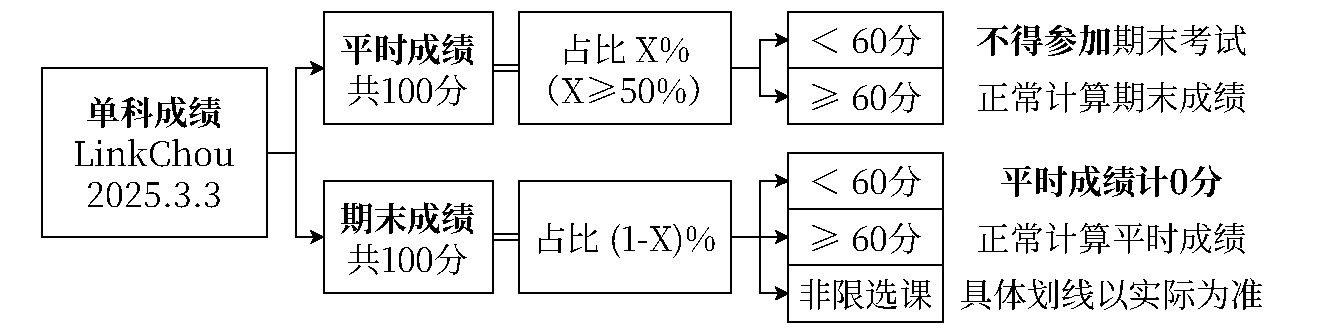
\includegraphics[width=\textwidth]{resources/sundry/单科成绩计算.pdf}
    \label{score}
\end{table}

\subsection[绩点]{绩点}
\label{gpa} % grade point average
\begin{enumerate}
    \item \textbf{平均学分绩点(GPA) ≥ 2}是获得学位证的要求之一
    \item 绩点计算方式如下:
          \begin{enumerate}
              \item \textbf{课程绩点}:(课程综合成绩 / 10)-- 5\\
                    注:综合成绩不及格绩点记为0分
              \item \textbf{平均学分绩点(GPA)}(平均绩点):
                    $$\frac{\sum (课程绩点 \cdot 课程学分)}{\sum 课程学分}$$
          \end{enumerate}
    \item 补考合格的科目按60分计,换算后为1绩点,其他特殊情景参考\uref{retake}小节
\end{enumerate}

\subsection[学分]{学分}
\begin{enumerate}
    \item 需修满对应的学分方可授予学位证
    \item 学分还用于学费计算(详见\uref{tuition}小节)
    \item 特殊事项:“公共选修课联盟”的公共选修课程不算学分、不收学费
    \item 各类学分要求详表\footnotemark 如下图所示
\end{enumerate}

\pagebreak[3]

\footnotetext{因不同学制、学院、年级要求各不相同,本图仅以\textbf{2021级临床医学院临床医学系普通5年制本科}为例,依照教务处\uhref{https://jwch.sdsmu.edu.cn/_upload/article/files/c5/2c/413ce30d4e259227f5b56e35410b/066fa55d-74ca-417e-b3b9-1af274317778.pdf}{《山东第二医科大学本科专业人才培养方案(2021版)》}制作,具体内容参见学生手册相关章节和教务处官网说明,如有变更恕不另行通知。}
\begin{table}[H]
    \centering
    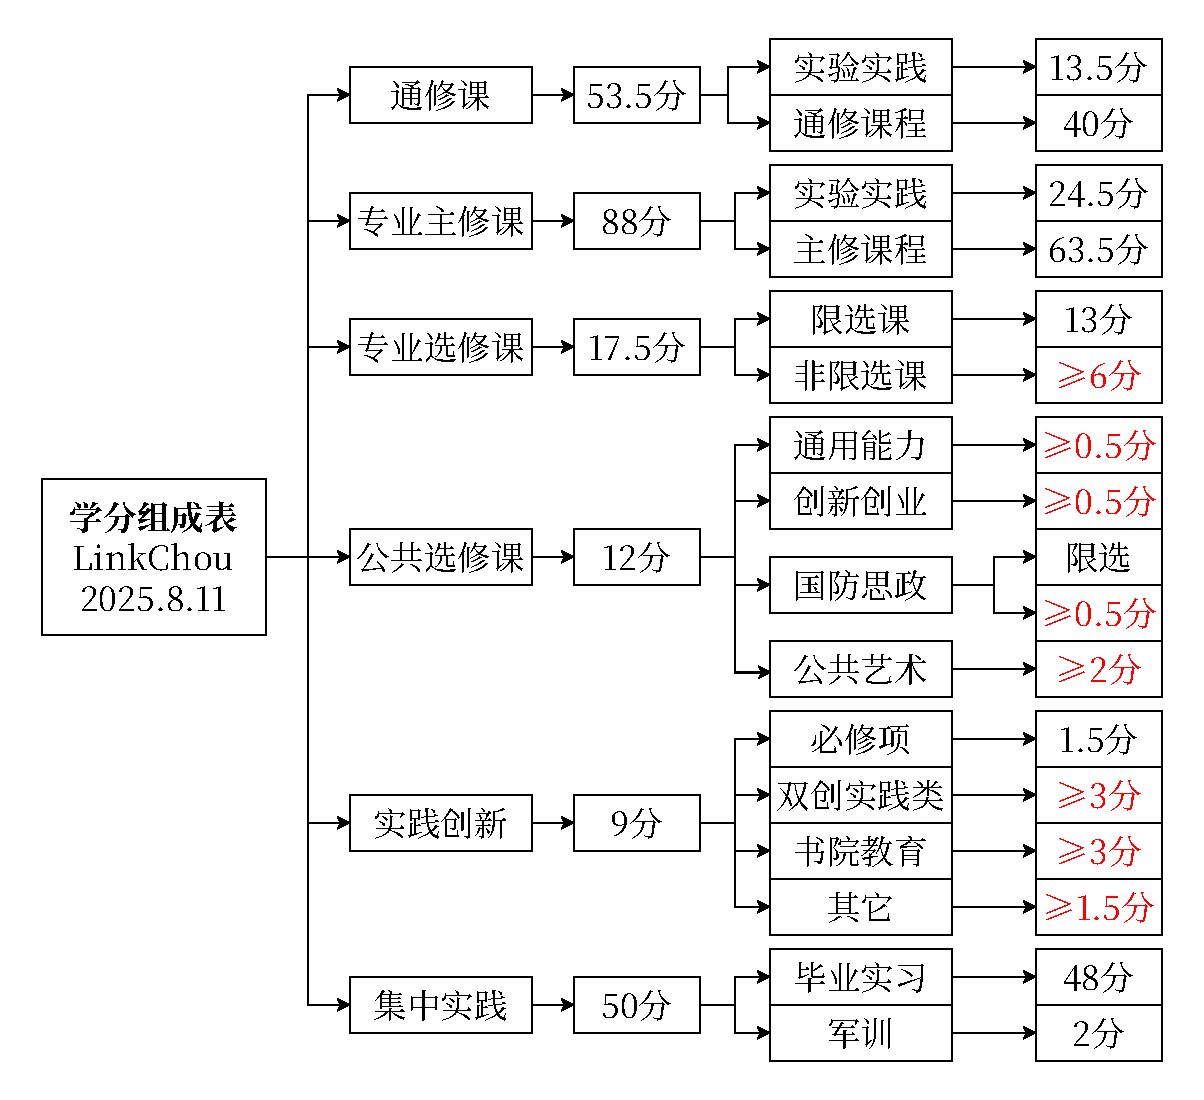
\includegraphics[width=\textwidth]{resources/sundry/学分.pdf}
    \label{credit}
\end{table}

\subsection[缓考、补考与重修]{缓考、补考与重修}
\label{retake}
注:本节内容摘编自《山东第二医科大学考试工作管理办法》第七章“缓考补考重修”与《山东第二医科大学课程重修管理办法》,如有不甚清晰之处请参照原文。

\subsubsection[补考]{补考}
\begin{enumerate}
    \item 必修课、限定选修课不及格(50 ≤ 分数 < 60)可以申请补考1次,仅计算卷面成绩,若及格则按60分计入综合成绩(折算为1绩点)
    \item 非限选课、公共选修课不及格需改选或重选,不予补考
    \item 每门课程仅1次补考机会(缺考除外),不额外收费
\end{enumerate}

\subsubsection[重修]{重修}
\begin{enumerate}
    \item 缓考或补考不及格者需要重修对应科目
    \item 必修课、限定选修课不及格(分数 < 50)需重修对应科目
    \item 非限选课、公共选修课不及格可以选择重修或直接改选其他科目
    \item 最终分数以实际为准(计入新的平时分)
\end{enumerate}

\subsubsection[缓考]{缓考}
缓考科目的分数以考试为准(计入平时分),缓考申请教程参见\uref{deferred_exam}


\subsection[关于选修课的补充说明]{关于选修课的补充说明}
\begin{enumerate}
    \item 选修课分专业选修和公共选修两大类(详见\uref{credit}),\textbf{推荐在大一全年、大二上学期就把各类选修学分全都修满},这样就不用在后面学业愈重的情况下兼顾选修课的学习了,可以专心针对专业课程进行深入学习
    \item 专业选修课有限选和非限选之分,限选的课程无需操心,教务系统会自动选课,只需要保证非限选的课程学分达标即可
    \item 公共选修课每一类都要选至少一门,且需要满足总分,其中部分类别还有额外要求(详见\uref{credit}),国防教育类有国家限选课程(到时候看具体通知,会说的很明白的)
    \item 公共选修课有一部分是在教室上的,还有一部分是线上课程(使用“知到”app进行学习,大多数有平时分,不能突击),可以根据自己的实际情况选择\footnotemark
          \footnotetext{一般来讲线下课好过,每星期去一次教室听听课就行,结课考试也很简单;但是线上课随时都能刷课,刷完课考完试就不用每周都去听课了,根据自己的需求选择。}
\end{enumerate}

\section[自习禁止事项]{自习禁止事项}
\begin{enumerate}
    \item \textbf{禁止在教室内亲嘴、喧哗、频繁说话}
    \item \textbf{禁止在自习室内抖腿}
    \item 禁止外放音乐、视频等
    \item 禁止在大服、非本班上课常用教室占座
    \item 禁止在教室内食用气味浓的食物(例如榴梿、辣条等)
    \item 禁止长时间占用教室内电源插座,仅允许应急充电
    \item 禁止在教室以及教室旁厕所内吸烟
\end{enumerate}

\section[其他说明]{其他说明}
\begin{enumerate}
    \item \textbf{有以下情况将无法获得学位证:}
          \begin{enumerate}
              \item 修不够每项对应的学分
              \item 平均绩点 < 2分
              \item 受过记过及以上处分
              \item 其他不符合相关要求的情况
          \end{enumerate}
    \item 累计两次获得三级学业预警的将会留级
    \item \textbf{大一不参与四六级,大二才能报名四六级考试}
    \item \textbf{\uul{转专业}\footnotemark:}
          \footnotetext{依据教务处2024年5月21日发布的\uhref{https://jwch.sdsmu.edu.cn/2024/0521/c2593a131550/page.htm}{《山东第二医科大学2024年普通全日制本科学生转专业工作方案》}以及《山东第二医科大学普通全日制本科学生转专业实施办法(修订)》简化,具体规定详见链接。该规定每年不一,如有变动,以教务处政策为准。}
          \begin{enumerate}
              \item 需满足以下条件:
                    \begin{enumerate}
                        \item 取得学籍的普通全日制一年级本科在校生
                        \item 未受处分、思想过硬、符合体检要求
                        \item 第一学年必修课和专业限定选修课平均成绩在本专业排名前30\%,且未挂科
                        \item 以特殊招生形式录取的学生,国家有相关规定或者录取前与学校有明确约定的(如公费医学生等),不得申请转专业
                    \end{enumerate}
              \item 考试科目:思政、英语\footnotemark、数学,比例为1:1:1,考试时间150分钟,总分为150分
                    \footnotetext{高考小语种考生可选择小语种替代英语,需在报名时备注,不备注者参加英语考试。}
              \item 流程:
                    \begin{enumerate}
                        \item 核算学生第一学年学习成绩并公示各类数据
                        \item 8月31日开始报名
                        \item 9月5日组织考试(地点详见相关通知)
                        \item 9月6日~10日公示录取名单\footnotemark
                              \footnotetext{按照“分数优先,遵循志愿,一次投档”的原则进行录取,成绩排名在专业应考人员中居前20\%者取得转专业资格。}
                        \item 9月11日~12日报到
                    \end{enumerate}
          \end{enumerate}
    \item 关于奖学金\footnotemark:本校有国家奖学金、校长奖学金、校级3等级奖学金等
          \footnotetext{请注意,目前学校仅能通过本人身份开通的、已开户的、账户已激活的、无异常的工商银行储蓄卡发放奖学金,详情政策可咨询学校财务处。}
    \item 新生开学考试\footnotemark 的内容为高中英语、高中数学,旨在让各位同学收心
          \footnotetext{按照往年惯例,不公布具体成绩。}
    \item \textbf{关于档案填写:}入档资料具有不能涂改、不能标记、不能修正的特性,因此严禁使用修正液或修正带对其涂改(涂改修正后立即作废)。填表时务必确保各类时间填写正确、与原始档案一致。此外,建议初次填写时使用铅笔轻轻填写,待负责人确认无误后方可擦除后使用黑色中性笔或中油笔填写(入档纸张为特殊A4纸,厚、重、滑,难以自行复印)
    \item 关于实验课与实验服(白大褂):在实验课上课时务必按要求正确洗手并佩戴头套、口罩、手套,着实验服,\textbf{\uul{严禁任何人在任何其它地点(尤其是餐厅)着实验服}!}因在实验室中需频繁接触实验动物、微生物,\textbf{极其推荐将实验课书包与普通课书包分开}!
          \label{schoolbag}
    \item 关于实验课:因为敏行楼实验室门牌号极其混乱,因此极其推荐提前20~30分钟前往确认教室地点,详情参见\uref{map_fuyanshan_minxing}处的敏行楼地图
\end{enumerate}

\section[早操、跑步打卡与晚自习]{早操、跑步打卡与晚自习}
\begin{enumerate}
    \item 早操时间一般为06:00~07:00,晚自习时间通常为19:00~21:00,教室22:00关闭
    \item 早操与晚自习贯穿整个大一\footnotemark,并且跑操与晚自习均有院系学生会不定时进行抽查出勤率等指标,最终结果计入班级综测(详见\uref{class_evaluation})的评分
          \footnotetext{按照惯例,麻醉专业无早操,只需要大一、大二早晨七点签到。}
    \item 学校已开始试行跑步打卡,详见相关通知
\end{enumerate}

\section[班级综测]{班级综测}
\label{class_evaluation}
\begin{enumerate}
    \item 综测是综合素质测评的简称,一般包含学习、活动、比赛等大类,加权相加后为得分,各年级要求不一,详见学生手册
    \item 班级综测是用于考核各班表现的评判指标,与班级评优评先、班集体评优评先名额分配、见习点分配\footnotemark 强相关,每学期计算一次,截至见习
          \footnotetext{以截至见习之前的各学期平均班级综测成绩计算班级排名,公费班级根据本年级政策进行。}
    \item 班级综测直接决定本班级同学后期学习和生活所在的医院规模、等级和生活条件,请大家务必重视\\
          例如:宿舍有无空调、暖气、洗衣机,是否提供插座,是否有早操和晚查寝\footnotemark 等
          \footnotetext{这意味着能否在外租房居住。}
\end{enumerate}

\section[临床医学专业三阶段综合考试]{临床医学专业三阶段综合考试}
大一的基础课程是一切的根基。

另注,本节内容参考《山东第二医科大学临床医学专业“三阶段”综合考试实施方案》编写而成。

\subsection[第一阶段综合考试(基础医学综合考试)]{第一阶段综合考试(基础医学综合考试)}
\begin{enumerate}
    \item 考察内容:组织胚胎学、病理学、病理生理学、解剖学、生理学、生物化学、药理学、医学免疫学、医学微生物学
    \item 考查时间与方式:第6学期进行,机考或笔试
    \item 其他信息:时长2.5小时,共300题,满分100分
\end{enumerate}

\begin{table}[H]
    \centering
    \begin{tblr}{
            cells = {c,m},
            rowhead = {1},
            row{1,Z} = {cmd=\bfseries},
            hline{1-2,Z} = {-}{1pt},
        }
        考试内容     & A1型题   & A2型题   & B1型题   & 总计     \\
        组织胚胎学   & 45~50\% & 35~40\% & 15~20\% & 5~10\%  \\
        病理学       & 45~50\% & 35~40\% & 15~20\% & 10~15\% \\
        病理生理学   & 45~50\% & 35~40\% & 15~20\% & 10~15\% \\
        解剖学       & 45~50\% & 35~40\% & 15~20\% & 10~15\% \\
        生理学       & 45~50\% & 35~40\% & 15~20\% & 10~15\% \\
        生物化学     & 45~50\% & 35~40\% & 15~20\% & 10~15\% \\
        药理学       & 45~50\% & 35~40\% & 15~20\% & 10~15\% \\  %避免自动换行不对劲导致出现vbox warning
        医学免疫学   & 45~50\% & 35~40\% & 15~20\% & 10~15\% \\
        医学微生物学 & 45~50\% & 35~40\% & 15~20\% & 10~15\% \\
        总计         & 45~50\% & 35~40\% & 15~20\% & 100\%
    \end{tblr}
\end{table}

\subsection[第二阶段综合考试(临床医学综合考试)]{第二阶段综合考试(临床医学综合考试)}
\begin{enumerate}
    \item 考察内容:
          \begin{enumerate}
              \item 理论考试:
                    \begin{enumerate}
                        \item 基础医学:病理学、解剖学、生理学、生物化学、药理学、医学免疫学、医学微生物学
                        \item 临床医学:内科学、外科学、妇产科学、儿科学
                        \item 医学人文:医学伦理学、医学心理学
                        \item 预防医学:预防医学
                    \end{enumerate}
              \item 技能考试:病史采集、体格检查、基本操作技能、沟通交流能力、人文关怀
          \end{enumerate}
    \item 详情考试形式、考试时间、试题数量以“国家医学考试中心”通知为准
    \item 下附往年二阶段理论考试详表
\end{enumerate}

\begin{tblr}[
        long,
        caption = {二阶段理论考试详表},
    ]{
        cells = {c,m},
        rowhead = {1},
        row{1,Z} = {cmd=\bfseries},
        hline{1-2,Z} = {-}{1pt},
    }
    考试内容 & A1型题   & A2型题   & B1型题   & 总计     \\
    基础医学 & 45~50\% & 35~40\% & 15~20\% & 40~45\% \\
    临床医学 & 20~25\% & 70~75\% & 3~5\%   & 40~45\% \\
    医学人文 & 45~50\% & 35~40\% & 15~20\% & 5~10\%  \\
    预防医学 & 35~40\% & 55~60\% & 3~5\%   & 5~10\%  \\
    总计     & 30~35\% & 50~55\% & 10~15\% & 100\%
\end{tblr}

\begin{tblr}[
        long,
        caption = {二阶段实践考试详表},
        note{1} = {沟通能力、人文关怀等医学人文素养的考核融合到各站,分值约占15\%。},
    ]{
        cells = {c,m},
        rowhead = {1},
        row{1,Z} = {cmd=\bfseries},
        hline{1-2,Z} = {-}{1pt},
    }
    考站 & 考试内容\TblrNote{1} & 考试方式 & 考试时间 & 分值 \\
    1站  & 病史采集             & SP       & 10分钟   & 20   \\
    2站  & 病史采集             & SP       & 10分钟   & 20   \\
    3站  & 体格检查             & 操作     & 10分钟   & 15   \\
    4站  & 体格检查             & 操作     & 10分钟   & 15   \\
    5站  & 基本操作             & 操作     & 10分钟   & 15   \\
    6站  & 基本操作             & 操作     & 10分钟   & 15   \\
    合计 &                      &          & 60分钟   & 100  \\
\end{tblr}


\subsection[第三阶段综合考试(毕业综合考试)]{第三阶段综合考试(毕业综合考试)}
\begin{enumerate}
    \item 考察内容:
          \begin{enumerate}
              \item 理论考试:内科学、外科学、妇产科学、儿科学
              \item 技能考试:职业素质、病史采集、体格检查、基本操作、辅助检查、病例分析
          \end{enumerate}
    \item 考查时间与方式:实习结束、毕业前进行,笔试或机考、面试
    \item 其他信息:理论考试时长2小时,共200题,满分100分;技能考试时长1小时,形式为客观结构化临床考试(OSCE),共12~16站,满分100分
\end{enumerate}

\begin{tblr}[
        long,
        caption = {三阶段理论考试详表},
    ]{
        cells = {c,m},
        rowhead = {1},
        row{1,Z} = {cmd=\bfseries},
        hline{1-2,Z} = {-}{1pt},
    }
    考试内容 & A1型题   & A2型题   & A3型题   & 总计     \\
    内科学   & 45~50\% & 25~30\% & 25~30\% & 35~40\% \\
    外科学   & 45~50\% & 25~30\% & 25~30\% & 35~40\% \\
    妇产科学 & 45~50\% & 25~30\% & 25~30\% & 10~15\% \\
    儿科学   & 45~50\% & 25~30\% & 25~30\% & 10~15\% \\
    总计     & 30~35\% & 50~55\% & 10~15\% & 100\%
\end{tblr}

\subsection[相关规定]{相关规定}
\begin{enumerate}
    \item 补考:一阶段由基础医学院组织补考;二阶段由教务处组织考试;三阶段由临床医学院组织补考
    \item 成绩折合与毕业:各阶段理论考试成绩按照2:4:4的比例折算后,作为毕业考试理论成绩;二、三阶段技能考试成绩按5:5折算后作为毕业考试技能成绩;不及格者不予毕业
    \item 综测与奖学金:一、二阶段成绩纳入个人综测和奖学金评定
    \item 实习:二阶段合格者可以进入医院实习,否则需要通过实践教学管理处和临床医学院组织的实习准入考试
\end{enumerate}
